\subsection{Directional Derivatives}%
\label{sec:directional-derivatives}
%%%%%%%%%%%%%%%%%%%%%%%%%%%%%%%%%%%%

\subsubsection{The Sorted \texorpdfstring{\(\ell_1\)}{l1}
  Norm}

\begin{theorem}
  \label{thm:sl1-directional-derivative}
  Let \(v \in \bbR^p \setminus \{0\}\), \(h_0 \in \big(0, \min_{i,j \in
    \{i : \beta_i \neq 0\}}\big| |\beta_i| - |\beta_j| \big|/\max_k|v_k| \big]\) and
  define \(\sigma\) to be the permutation such that
  \[
    |\beta + h_0v|_{\sigma(1)} \geq |\beta + h_0v |_{\sigma(2)}
    \geq \cdots \geq |\beta + h_0v|_{\sigma(p)}.
  \]
  \mm{I think we need to state that for any \(h \leq h_0\), \(\sigma\) is still a correct reordering for \(\beta + h v\) (that we use at the last line of \eqref{eq:sl1-directional-derivative})}
  The directional derivative for the sorted \(\ell_1\) norm, \(J(\beta)\), is
  \[
    D_v J(\beta) =
    \sum_{i=1}^m \sum_{j \in \mathcal{C}_i} \lambda_j v_{\sigma(j)}\sign(\beta_{\sigma(j)} + h_0v_{\sigma(j)})\]
  \mm{doesn't the definition of \(h_0\) imply that \(\beta_j + h_0 v_j\) has the sign of \(\beta_j\)?}
  \jl{Not when \(\beta = 0\), since then the sign is determined solely by \(v\).}
  where
  \[
    \mathcal{C}_i = \{j : |\beta_j| = c_i\},\qquad
    c_1 > c_2 > \cdots > c_m \geq 0.
  \]
\end{theorem}
\begin{proof}
  The directional derivative for the sorted \(\ell_1\) norm and a direction
  \(v\) with \(\lVert v \rVert = 1\) \mm{is normalization needed?}\jw{No, but I think we should put in the definition of Theorem, as it no limitation?} is
  \begin{equation}
    \label{eq:sl1-directional-derivative}
    \begin{aligned}
      D_v J(\beta) & = \lim_{h \searrow 0} \frac{J(\beta + h v) - J(\beta)}{h}                                                                     \\
                   & = \lim_{h \searrow 0} \frac{\sum_{j=1}^p\lambda_j\big(|\beta + vh|_{\sigma(j)} - |\beta|_{(j)}\big)}{h}                       \\
                   & = \lim_{h \searrow 0}\frac{\sum_i \sum_{j \in \mathcal{C}_i} \lambda_j\big(|\beta + vh|_{\sigma(j)} - |\beta|_{(j)}\big)}{h}. \\
    \end{aligned}
  \end{equation}
  Assume without loss of generality that \(c_m = 0\).
  Then
  \[
    \sum_{j \in \mathcal{C}_m}\frac{\lambda_j \big( |\beta + vh|_{\sigma(j)} - |\beta|_{(j)}\big)}{h}
    = \sum_{j \in \mathcal{C}_m} \lambda_j \sign(\beta + hv)_{\sigma(j)}v_{\sigma(j)}.
  \]
  Next, recall the construction of \(h_0\) and
  observe that \(\sign(\beta_j + hv_j) = \sign(\beta_j)\)
  and \(\sigma(j) = (j)\) for all \(j \notin \mathcal{C}_m\) \mm{here there is an issue for me because, by the clustering effect, \(()\) is not uniquely defined. Since \(v\) allows each component of \(\beta + h v\) to move at different speed, we may, inside each cluster, end up with any arbitrary order (the limit on the magnitude of \(h\) only imposes that values from one cluster don't end up crossing another cluster )}\jw{I don't follow. You have an arbitrary ordering if \(|\beta_i +hv_i|\) and \(|\beta_j +hv_j|\) otherwise the ordering is defined by \(\sigma\) as it determined by \(\beta\) and \(v\)?}
  \mathurin{It's a small detail, but neither \(\sigma\) nor \(()\) are uniquely defined.
    For me the above sentence says that for \(h\) small enough and the non zero clusters, \(\sigma\) does not depend on \(v\). But if you take \(\beta = (0, 10, 10, 20)\) and \(hv = (0, 1, 0, 0)\) or \(hv = (0, 0, 1, 0)\), they don't yield the same \(\sigma\).
    I'm thinking a rigorous formulation is: "\(\sigma\) is a valid reordering for \(\beta\)"}
  whenever \(0 < h < h_0\).
  It follows that
  \[
    \sum_{j \in \mathcal{C}_i} \frac{\lambda_j\big(|\beta + hv|_{\sigma(j)} - |\beta|_{(j)}\big)}{h}
    = \sum_{j \in \mathcal{C}_i} \lambda_j\sign(\beta + vh)_{\sigma(j)}v_{\sigma(j)}.
  \]
  From this, we see that \eqref{eq:sl1-directional-derivative} reduces to
  \[
    \lim_{h \searrow 0} \sum_i \sum_{j \in \mathcal{C}_i} \lambda_j\sign(\beta + vh)_{\sigma(j)}v_{\sigma(j)}
    = \sum_i \sum_{j \in \mathcal{C}_i} \lambda_j\sign(\beta + vh_0)_{\sigma(j)}v_{\sigma(j)}.
  \]
  \mathurin{Is this reformulation equivalent? (provided \(c_m = 0\))}
  \JL{Yes, good point! But we still need \(h_0\) for the permutation.}
  Then it follows that
  \begin{equation*}
    D_v J(\beta) = \sum_{j \notin \cC_m} \lambda_j \sign (\beta_{\sigma(j)}) v_{\sigma(j)}
    +
    \sum_{j \in \cC_m} \lambda_j \sign (v_{\sigma(j)}) v_{\sigma(j)}.
  \end{equation*}
\end{proof}

\begin{remark}
  Using \cref{thm:sl1-directional-derivative}, we see that
  the directional derivative for \eqref{pb:slope} is
  \[
    D_v P(\beta) = v^T \big(\nabla L(\beta)\big) + D_v J(\beta).
  \]
\end{remark}

\subsubsection{Alternative Formulation}

An alternative formulation (with identical solution) is to minimize
\[
  \begin{aligned}
    P(c_k) & = \frac{1}{2} \lVert y - X_{\bar{\mathcal{C}_k}} \beta_{\bar{\mathcal{C}_k}} - \big(X_{\mathcal{C}_k} \beta_{\mathcal{C}_k}\big)c_k  \rVert_2^2 + \sum_{j \notin {\mathcal{C}_k}} \lambda_{(j)^-}|\beta_k| + |c_k|\bigg(\sum_{j \in {\mathcal{C}_k}} \lambda_{(j)^- }|\beta_j|\bigg),
  \end{aligned}
\]
and \(\beta_k := c_k\beta_k\).


\subsubsection{Subgradient}

\begin{theorem}\label{thm:cluster-subdifferential}
  Let \(\beta\) be a fixed vector and \(p_i\) and \(c_i\) be the size and
  coefficient, respectively, of the \(i\)th cluster in \(\beta\).
  Next, let \(\beta(z)\) be defined as in \eqref{eq:coordinate-update-beta}
  and \(a\) and \(b\) be vectors of indexes, such that
  \(a_i\) and \(b_i\) are the first and last indexes, respectively,
  of the \(\lambda\) sequence associated with the \(i\)th cluster
  in \(B(z)\). The subdifferential for \(J_k(z)\) at \(z\) is
  then
  \[
    \partial_{z} J_k(z) =
    \begin{cases}
      \big[-\sum_{j = p - p_k + 1}^{p}\lambda_j, \sum_{j = p - p_k + 1}^{p}\lambda_j\big]                         & \text{if } z = 0 \neq c_m,  \\
      \big[-\sum_{j = p - p_m + 1}^{p - p_m + p_k}\lambda_j, \sum_{j = p - p_m + 1}^{p - p_m + p_k}\lambda_j\big] & \text{if } z = 0 = c_m,     \\
      \big[\sum_{j = b_i - p_k + 1}^{b_i}\lambda_j, \sum_{j = a_i}^{a_i + p_k} \lambda_j\big]                     & \text{if } z = c_i \neq 0,  \\
      \big[-\sum_{j = a_i}^{a_i + p_k} \lambda_j, -\sum_{j = b_i - p_k + 1}^{b_i}\lambda_j\big]                   & \text{if } z = -c_i \neq 0, \\
      \sign(z)\sum_{j \in C(z)} \lambda_{(j)^-_z}                                                                 & \text{otherwise.}           \\
    \end{cases}
  \]
\end{theorem}
\begin{proof}
  Since \(J_k(z)\) is convex, \(g \in \mathbb{R}\) is a
  subgradient at \(z\) if and only if~\cite[Theorem 23.2]{rockafellar1970}
  \begin{equation}
    \label{eq:subgrad-ineq}
    J'(x; \delta) \geq g\delta \qquad \forall\,\delta \in \{-1, 1\}.
  \end{equation}
  Starting with the case \(z = 0 \neq c_m\), we have
  \[
    \begin{aligned}
       & |\delta| \smashoperator{\sum_{j \in C(\varepsilon\delta)}} \lambda_{(j)^-_{\varepsilon\delta}} \geq \delta g     & \implies \\
       & \sign(\delta) \smashoperator{\sum_{j \in C(\varepsilon\delta)}} \lambda_{(j)^-_{\varepsilon\delta}} \geq g       & \implies \\
       & -\smashoperator{\sum_{j = p - p_k + 1}^p} \lambda_j \leq g \leq \smashoperator{\sum_{j=p - p_k + 1}^p} \lambda_j
    \end{aligned}
  \]
  since \(C(\varepsilon\delta) = C(0)\) in this case.

  In the case \(z = 0 = c_m\), the cluster \(C(\varepsilon\delta)\) will occupy the
  next-to-last spot in the order permutation, and hence
  \[
    -\smashoperator{\sum_{j = p - p_k - p_m + 1}^{p - p_m}} \lambda_j
    \quad \leq g \leq \quad
    \smashoperator{\sum_{j=p - p_k - p_m + 1}^{p - p_m}} \lambda_j.
  \]

  In the case \(z = c_i\),~\eqref{eq:subgrad-ineq} corresponds to
  \begin{equation}
    \label{eq:subgrad-ineq-nonzero}
    \sign(z)\delta \smashoperator{\sum_{j \in C(z + \varepsilon\delta)}} \lambda_{(j)^-_{z + \varepsilon\delta}} \geq \delta g.
  \end{equation}
  For \(z > 0\), \(\delta = 1\), \(C(z + \varepsilon\delta)\) will occupy the position
  in the order permutation of \(B(z + \varepsilon\delta)\) that precedes the \(i\)th
  cluster, and hence
  \begin{equation*}
    \sign(z)\delta \smashoperator{\sum_{j \in C(z + \varepsilon\delta)}} \lambda_{(j)^-_{z + \varepsilon\delta}} \geq \delta g
    \implies
    \smashoperator{\sum_{j \in C(z + \varepsilon\delta)}} \lambda_{(j)^-_{z + \varepsilon\delta}} \geq g \implies
    \smashoperator{\sum_{j = a_i}^{a_i + p_k}} \lambda_j \geq g.
  \end{equation*}
  If \(\delta = -1\), then \(C(z + \varepsilon\delta)\) instead occupies the
  position succeeding the \(i\)th cluster, and we have
  \begin{equation*}
    \sign(z)\delta \smashoperator{\sum_{j \in C(z + \varepsilon\delta)}} \lambda_{(j)^-_{z + \varepsilon\delta}} \geq \delta g
    \implies
    -\smashoperator{\sum_{j \in C(z + \varepsilon\delta)}} \lambda_{(j)^-_{z + \varepsilon\delta}} \geq -g \implies
    \smashoperator{\sum_{j = b_i - p_k + 1}^{b_i}} \lambda_j \leq g.
  \end{equation*}
  It is easy to see that for \(z_i = c_i < 0\), we must analogously have
  \[
    -\smashoperator{\sum_{j = b_i - p_k + 1}^{b_i}} \lambda_j
    \leq g \leq
    \smashoperator{\sum_{j = a_i}^{a_i + p_k}} \lambda_j.
  \]
  For all other \(z\), \(J_k\) is differentiable and therefore
  \[
    \partial J_k(z) = \sign(z) \smashoperator{\sum_{j \in C(z)}} \lambda_{(j)^-_z}.
  \]
\end{proof}

The objective and subgradient for the cluster-wise problem are shown in
\cref{fig:cluster-grad-obj}.

\begin{figure}[htbp]
  \centering
  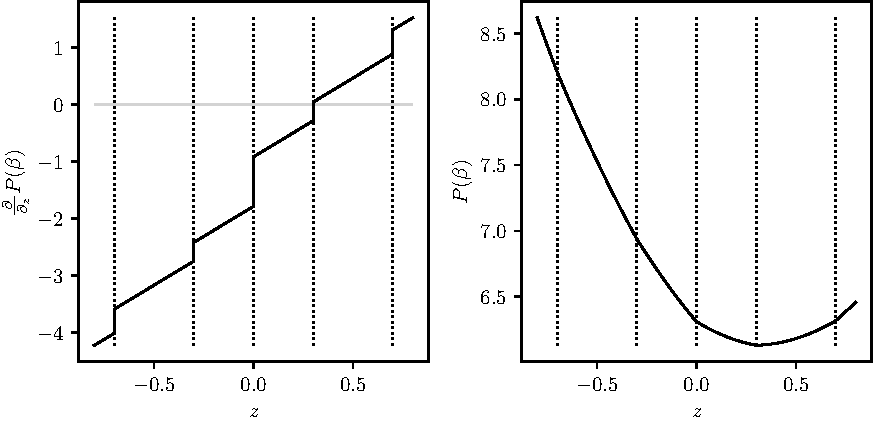
\includegraphics[]{clusterupdate-grad-obj}
  \caption{%
    Objective and gradient under the constraint that we have a fixed
    cluster.
    The optimum is found at \(\alpha = 0.3\).
  }%
  \label{fig:cluster-grad-obj}
\end{figure}

We are now ready to introduce a solution to~\eqref{eq:cluster-problem}, using
the SLOPE thresholding operator~\cref{thm:slope-thresholding}.

\begin{theorem}
  \label{thm:slope-thresholding}
  Let
  \begin{multline*}
    T_k(\gamma, \omega; c, \lambda) = \\
    \begin{cases}
      0                                                                         &
      \splitfrac{
        \text{if } \big(-\sum_{j = p - p_k + 1}^p \lambda_j < \gamma \leq \sum_{j = p - p_k + 1}^p \lambda_j
        \text{ and } c_m \neq 0\big)
      }{%
        \text{ or } \big(  -\sum_{j = p - p_k - p_m + 1}^{p - p_m} \lambda_j < \gamma \leq \sum_{j = p - p_k + 1}^{p_m} \lambda_j \text{ and } c_m = 0\big),
      }                                                                                                                                                                                                                    \\
      c_i                                                                       & \text{if } \exists\, i \neq k: \sum_{j = b_i - p_k + 1}^{b_i} \lambda_j \leq \gamma - \omega c_i \leq \sum_{j = a_i}^{p_k} \lambda_j,    \\
      -c_i                                                                      & \text{if } \exists\, i \neq k : \sum_{j = b_i - p_k + 1}^{b_i} \lambda_j \leq - \gamma - \omega c_i \leq \sum_{j = a_i}^{p_k} \lambda_j, \\
      \frac{1}{\omega}\left(\gamma - \sum_{j \in C(z)} \lambda_{(j)^-_z}\right) & \text{otherwise.}                                                                                                                        \\
    \end{cases}
  \end{multline*}
  A minimizer for \eqref{eq:cluster-problem} is given by \(T_k(\tilde{r}^T\tilde{x}, \tilde{x}^T\tilde{x}; c, \lambda)\).
\end{theorem}
\begin{proof}
  Let \(\gamma = \tilde{r}^T\tilde{x}\) and \(\omega = \tilde{x}^T\tilde{x}\).
  For a minimizer to~\eqref{eq:cluster-problem}, the optimality condition is
  \[
    0 \in \tilde{x}^T\tilde{x} z - \tilde{r}^T \tilde{x} + \partial J_k(z).
  \]
  \(z = c_i \neq 0\) is a minimizer of~\eqref{eq:cluster-problem} if and only if
  \[
    0 \in \omega c_i - \gamma +
    \left[\sum_{j = b_i - p_k + 1}^{b_i} \lambda_j, \sum_{j=a_i}^{p_k}\lambda_j \right],
  \]
  which is equivalent to
  \[
    \smashoperator[r]{\sum_{j = b_i - p_k + 1}^{b_i}} \lambda_j \leq \gamma - \omega c_i \leq \sum_{j = a_i}^{p_k} \lambda_j.
  \]
  \(z = -c_i \neq 0\) is a minimizer of~\eqref{eq:cluster-problem} if and only if
  \[
    0 \in -\omega c_i - \gamma +
    \left[-\sum_{j=a_i}^{p_k}\lambda_j, -\smashoperator{\sum_{j = b_i - p_k + 1}^{b_i}} \lambda_j\,\right],
  \]
  which is equivalent to
  \[
    \smashoperator[r]{\sum_{j = b_i - p_k + 1}^{b_i}} \lambda_j \leq -\gamma - \omega c_i \leq \sum_{j = a_i}^{p_k} \lambda_j.
  \]
  If \(c_m \neq 0\), then \(z = 0\) is a minimizer if
  \[
    0 \in -\gamma +
    \left[-\sum_{j = p - p_k + 1}^{p} \lambda_j, \sum_{j=p - p_k + 1}^{p}\lambda_j \right],
  \]
  which is equivalent to
  \[
    -\sum_{j = p - p_k + 1}^{p} \lambda_j \leq \gamma \leq \sum_{j = p - p_k + 1}^{p} \lambda_j.
  \]
  Finally, if \(c_m = 0\), then \(z = 0\) is a minimizer if
  \[
    0 \in -\gamma +
    \left[
      -\sum_{j = p - p_k - p_m + 1}^{p - p_m} \lambda_j,
      \sum_{j=p - p_k - p_m + 1}^{p - p_m}\lambda_j
      \right],
  \]
  which is equivalent to
  \[
    -\sum_{j = p - p_k + 1}^{p} \lambda_j \leq \gamma \leq \sum_{j = p - p_k + 1}^{p} \lambda_j.
  \]


